\chapter{Eksperyment z wykorzystaniem wahadła reakcyjnego}
\label{cha:pendulum}
\section{Opis problemu}
\label{sec:pendulum_description}
Wahadło reakcyjne to przykład jednego z~prostych układów nieliniowych. Na~końcu wahadła znajduje się tarcza, która może obracać się wokół osi równoległej do~osi obrotu wahadła (rysunek \ref{fig:pendulum_picture}). Jest ona wprawiana w~ruch przez silnik prądu stałego. Generowany w~ten sposób moment sprzęgający może być wykorzystany do~sterowania układem. \par
\begin{figure}
	\centering
	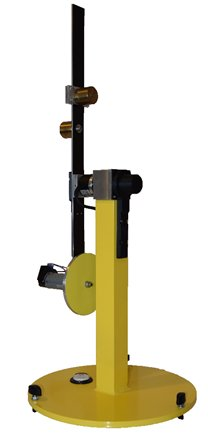
\includegraphics[width=0.4\linewidth]{pendulum.jpg}
	\caption{Wahadło reakcyjne \cite{Pendulum_picture}}
	\label{fig:pendulum_picture}
\end{figure}
Wahadło reakcyjne użyte w~pracy składało się z~następujących elementów:
\begin{itemize}
	\item Elementy mechaniczne
	\item Silnik prądu stałego sterowany za~pomocą PWM
	\item Dwa enkodery inkrementalne, jeden mierzący kąt obracającej się tarczy, drugi wykonujący pomiar kąta wychylenia wahadła
	\item Przeciwwaga pozwalająca na~zmianę wartości parametrów wahadła
	\item Skrzynka zasilania zawierająca zasilacz, wzmacniacze mocy i~jednostkę kondycjonowania sygnału
\end{itemize}
Model obiektu może być opisany równaniami:
\begin{align}
\label{eq:pendulum_model}
&\ddot{\theta} + 2\xi\omega_0\dot{\theta} + \omega_0^2 \sin \theta = k_p(u - H(\omega_t)) \nonumber \\
&\dot{\omega_t} = K(u - H(\omega_t)) 
\end{align}
gdzie $\theta$ to kąt wychylenia wahadła, $\omega_t$ to prędkość obrotowa tarczy, $u$ to wartość sterowania, natomiast pozostałe parametry wyznaczone eksperymentalnie w~\cite{Pendulum_report} przedstawiono w~tabeli \ref{tab:pendulum_params}.
\begin{table}[]
	\caption{Parametry modelu wahadła reakcyjnego}
	\label{tab:pendulum_params}
	\begin{center}
		\begin{tabular}{|l|l|l|l|l|}
			\hline
			\textbf{$\xi$} & \textbf{$\omega_0$} & \textbf{$K$} & \textbf{$k_p$} & \textbf{$H(\omega_t)$}\\ 
			\hline
			$0.03$ & $2.36$ & $529.798$ & $-4.3434$ & $0.0022\omega_t$ \\
			\hline
		\end{tabular}
	\end{center}
\end{table}
Model procesu otrzymano przekształcając model \ref{eq:pendulum_model} na~dyskretne równanie stanu oraz uwzględniając addytywny szum procesu:
\begin{align}
\label{eq:pendulum_process_model}
\theta(t+1) &= \theta(t) + T\omega(t) + w_1(t) \nonumber \\
\omega(t+1) &= \omega(t) - 2T\xi\omega_0\omega(t) - T\omega_0^2\sin (\theta(t)) + Tk_p(u - H(\omega_t(t))) + w_2(t) \nonumber \\
\theta_t(t+1) &= \theta_t(t) + T\omega_t(t) + w_3(t) \nonumber \\
\omega_t(t+1) &= \omega_t(t) + TK(u - H(\omega_t(t))) + w_4(t) 
\end{align}
dla stanu układu $\boldsymbol{x} = \begin{bmatrix}
\theta & \omega & \theta_t & \omega_t
\end{bmatrix}^T$, gdzie: $\theta$ - kąt wychylenia wahadła, $\omega$ - prędkość kątowa wahadła, $\theta_t$ - położenie tarczy, $\omega_t$ - prędkość kątowa tarczy, $\boldsymbol{w} \sim \mathcal{N}(\boldsymbol{0}, \boldsymbol{Q})$. 
\par
Model pomiarowy zakładał pomiar współrzędnych położenia środka tarczy względem osi obrotu wahadła:
\begin{align}
\label{eq:pendulum_measurement_model}
z_1(t) = r \sin (\theta(t)) + v_1(t) \nonumber \\
z_2(t) = r \cos (\theta(t)) + v_2(t)
\end{align}
dla odległości pomiędzy osią obrotu wahadła, a~środkiem tarczy $r=18\,cm$ oraz dla szumu pomiarowego $\boldsymbol{v} \sim \mathcal{N}(\boldsymbol{0}, \boldsymbol{R})$.
\section{Przebieg eksperymentu i przygotowanie danych}
\label{sec:pendulum_experiment}
Przy użyciu wahadła reakcyjnego wykonano eksperyment, podczas którego na~wahadło podawano prostokątny sygnał sterujący pobudzając obiekt do~ruchu oraz rejestrowano ruch wahadła za~pomocą kamery. Wartości sterowania oraz uznane za~wzorcowe wartości kąta wychylenia wahadła z~enkodera inkrementalnego zapisywane były na~komputerze z~wykorzystaniem środowiska MATLAB/Simulink. W~celu łatwego wykrycia środka tarczy, na~obiekcie umieszczono świecącą diodę. Synchronizacja klatek z~kamery oraz wartości zapisanych na~komputerze była natomiast możliwa dzięki umieszczeniu w~kadrze przebiegu wartości sterowania poruszającego tarczą. Przebieg eksperymentu pokazano na~rysunku \ref{fig:pendulum_experiment}.
\begin{figure}
	\centering
	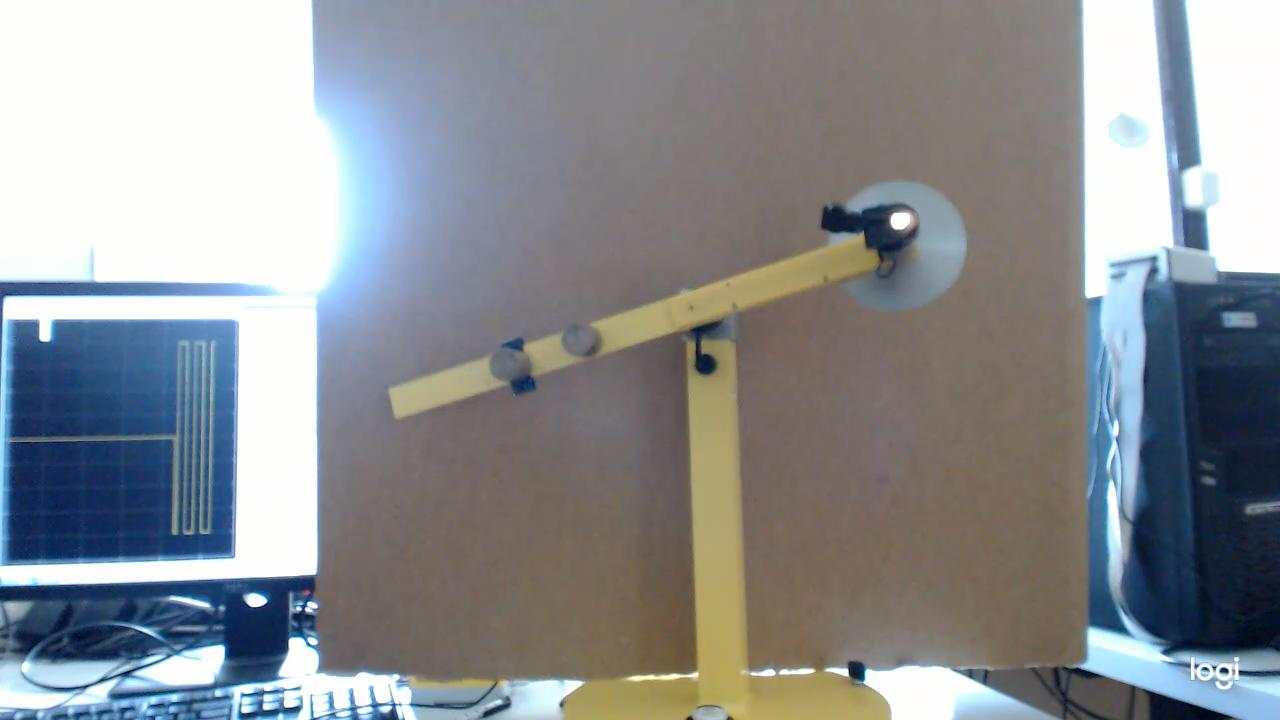
\includegraphics[width=0.8\linewidth]{pendulum_experiment.jpg}
	\caption{Przebieg eksperymentu z~wykorzystaniem wahadła reakcyjnego}
	\label{fig:pendulum_experiment}
\end{figure} \par
Po~wykonaniu eksperymentu, otrzymane dane zostały przetworzone w~środowisku MATLAB w~celu wykrycia istotnych informacji. Wykrycie świecącej diody umożliwiła binaryzacja ze~stałym progiem, wykonana na~klatkach w~skali szarości. Następnie obliczano środek ciężkości wykrytych pikseli w~obszarze ruchu wahadła, otrzymując współrzędne środka tarczy. Otrzymane współrzędne na~klatce filmu należało przeliczyć na współrzędne w~rzeczywistości. W~tym celu skorzystano z~transformacji płaskiej metodą DLT (ang. \textit{Direct Linear Transform}), opisaną w~\cite{DLT_description}. Równanie \ref{eq:DLT_transform} przedstawia transformację prowadzącą ze~współrzędnych $x$ i~$y$ w~płaszczyźnie wahadła, do~współrzędnych $u$ i~$v$ na~zdjęciu. 
\begin{align}
\label{eq:DLT_transform}
u &= \frac{M_1x + M_2y + M_3}{M_7x + M_8y + 1} \nonumber \\
v &= \frac{M_4x + M_5y + M_6}{M_7x + M_8y + 1}
\end{align}
Do~znalezienia współczynników występujących w~transformacji wykorzystano płaski obiekt o~znanej geometrii, umieszczony w~płaszczyźnie ruchu wahadła (rysunek \ref{fig:calibration}).
\begin{figure}
	\centering
	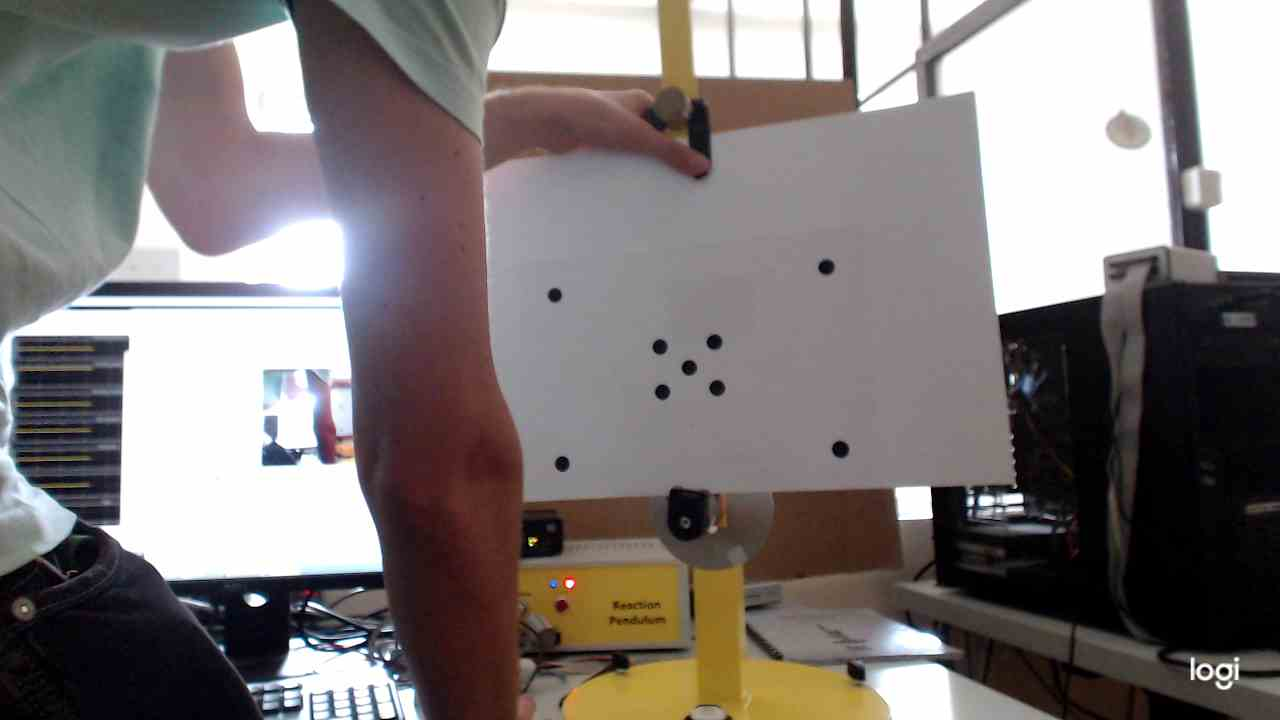
\includegraphics[width=0.8\linewidth]{calibration.jpg}
	\caption{Zdjęcie wykorzystane do kalibracji kamery metodą DLT}
	\label{fig:calibration}
\end{figure} \par
\section{Omówienie wyników}
\label{sec:pendulum_results}
Dane zebrane podczas eksperymentu przefiltrowano przy użyciu algorytmu rozszerzonego filtru Kalmana oraz filtru Kalmana Gaussa-Hermite'a stopnia trzeciego. Przyjęto następujące wartości parametrów filtracji: $\boldsymbol{x}(0|0) = \begin{bmatrix}
0 & 0 & 0 & 0
\end{bmatrix}^T$, $\boldsymbol{P}(0|0)=\boldsymbol{I}_{4\times4}$, $\boldsymbol{Q} = diag(0, 1, 0, 1)$, $\boldsymbol{R}=\boldsymbol{I}_{2\times2}$, $T=0.033\,s$. Rysunek \ref{fig:pendulum_results} przedstawia rezultaty filtracji algorytmami EKF oraz GHKF-3. Po~początkowym sporym błędzie występującym w~czasie, kiedy wahadło pozostawało w~bezruchu, estymata kąta wychylenia uzyskana przez algorytmy jest zbliżona do~wartości odczytanych z~enkodera. Różnica między algorytmami dla postawionego problemu okazała się bardzo niewielka, RMSE dla rozszerzonego filtru Kalmana wyniosło 0.23780, natomiast dla filtru Kalmana Gaussa-Hermite'a 0.23783. 
\begin{figure}
	\centering
	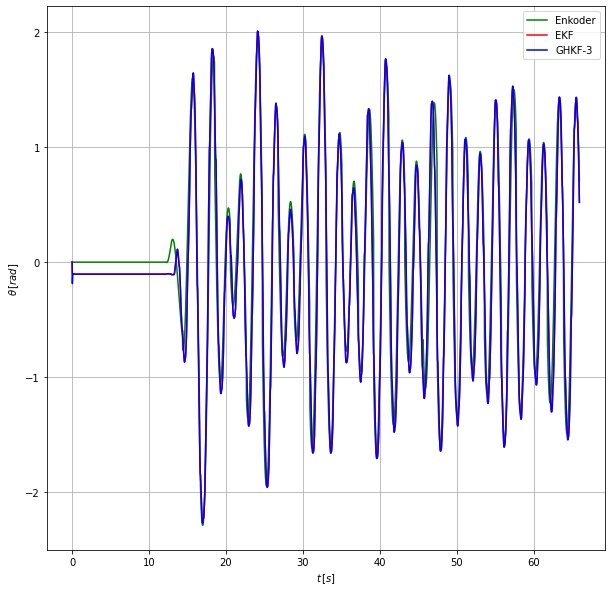
\includegraphics[width=0.8\linewidth]{pendulum_results.jpg}
	\caption{Wartości kąta wychylenia wahadła reakcyjnego}
	\label{fig:pendulum_results}
\end{figure}
